\documentclass[format=acmsmall, review=false]{acmart}

\usepackage{acm-ec-18}

\usepackage{booktabs} % For formal tables

\usepackage{textgreek}

\usepackage[ruled]{algorithm2e} % For algorithms

\usepackage{ textcomp }
\usepackage[demo]{graphicx}

\renewcommand{\algorithmcfname}{ALGORITHM}
\SetAlFnt{\small}
\SetAlCapFnt{\small}
\SetAlCapNameFnt{\small}
\SetAlCapHSkip{0pt}
\IncMargin{-\parindent}
\newcommand\mycommfont[1]{\footnotesize\upshape\textcolor{blue}{#1}}
\SetCommentSty{mycommfont}

\begin{document}
% Title portion. Note the short title for running heads 
\title[Novel algorithms for dynamic kidney exchange]{Novel algorithms for dynamic kidney exchange}  
\author{Submission 42}

% note that the abstract must come before \maketitle
\begin{abstract}
In recent years, kidney paired donation (KPD) has emerged as an alternative for end-stage renal disease patients with incompatible living donors. However, we argue that a larger number of patients may be reached if kidney transplant centers take into consideration how their pool of patients and donors will evolve over time. To that end, we contribute to the matching literature in dynamic settings by proposing two novel kidney exchange methods, and empirically evaluate these methods using simulations. Our objective function is the average number of matched patients per period. We restrict our experiments to pairwise kidney exchange, but the methods described here are easily extensible, computational constraints permitting. We find that at least one of our methods, based on multi-armed bandit algorithms, is able to outperform the myopic method that is used by kidney transplants in practice, sometimes by as much as 4\%.
\end{abstract}

% note: this command has been disabled to remove the ACM copyright block. Sorry...
%\thanks{This work is supported by the National Science Foundation,
%  under grant CNS-0435060, grant CCR-0325197 and grant EN-CS-0329609.}

\maketitle

\section{Introduction}

Patients suffering from end-stage renal disease have two available treatments: dialysis and renal transplant. While transplant is associated with ``lower mortality rates and improved quality of life compared to chronic dialysis treatment" \citep{tonelli2011systematic}, severe kidney shortage prevents tens of thousands of patients every year from receiving a transplant. In the US alone, there are currently over 90,000 patients in the kidney transplant waiting list, and patients often must wait several years before finding an available donor.

In order to overcome this challenge, in recent years \emph{kidney paired donation} (KPD) has emerged as an alternative option for patients who have an incompatible but otherwise willing living donor. The approach involves pooling patient-donor pairs and swapping or exchanging donors so as to increase the overall number of matched patients.

Kidney paired donation was proposed about three decades ago by \cite{rapaport1986case}, but its implementation in the United States began only in the early 2000s. At the same time, \cite{roth2004kidney} helped elevate KPD as an object of academic study, and since then it has evolved and expanded rapidly both in academic and outside of it. \citep{sonmez2013market}.

Nevertheless, even today the amount of kidney exchanges remains smaller than its potential, due to several reasons. As we will argue in this paper, one source of inefficiency in kidney exchange is that most transplant centers do not take into consideration the evolution of their kidney pool over time and, as we will demonstrate shortly via simulations, this can lead to large losses in terms of the overall number of pairs matched over time.

To this end we contribute to the \emph{dynamic} kidney matching literature by introducing two novel algorithms for kidney exchange. They are explained next.

\paragraph{\textbf{Main idea}} We propose two novel approaches for increasing the cardinality of matched pairs in a discrete-time dynamic model of kidney exchange: the \emph{direction prediction} and the \emph{multi-armed-bandit} methods. We also empirically evaluated these methods using simulations, under a variety of data-generating processes that we call \emph{environments}. 

Let's see how these methods work, and some of the challenges they overcome.

First, our \emph{direct prediction} method recasts the dynamic kidney exchange problem as a binary classification task: for each pair in the pool, we predict a binary label representing whether they should be matched today (one), or left for the future (zero), given their observable characteristics. The estimator used here was trained in data extracted from simulations under a variety of setups.

The main challenge with this approach is how to represent the data: while covariates such as ABO bloody type and current waiting time can be naturally represented by real numbers, it is not immediately clear how to represent their relationship to other nodes in the graph.  We attempt to overcome this issue by augmenting the data set with graph-theoretic notions such as measures of node centrality, size of graph, average degree, and so on. 

Our second method, named the \emph{multi-armed bandit} method, uses simulations to answer the question: ``if we take a particular action today, how likely are we to decrease the number of matched pairs between now and a horizon $h$?". Naturally, actions for which this probability is large should be left for the future, while actions for which this probability is low should be prioritized. The main challenge here is that simulations are so computationally costly, and the number of available actions so vast, that we are cannot realistically produce accurate estimates of this probability for all points in the action space. To overcome this issue, we employ multi-armed bandit (MAB) algorithms. Their role is to manage a relatively small computational budget and determine which actions are likely attractive (and should be explored further), and which are not (and thus not worth exploring much).


\paragraph{\textbf{Main results}} Our methods are evaluated via simulations. The simulation setups, which we call \emph{environments}, are inspired by models used the kidney exchange literature, and differ by their rules regarding blood- and tissue-type compatibility.

We have to benchmarks against which we compare our methods. First, a \textsc{myopic} algorithm that clears the maximal matching at each period. This benchmarks represents roughly what most organ clearinghouses are doing today. Second, in order to know what is the maximal payoff we could have achieve, had we been able to know the future, we also compare to an infeasible offline optimal algorithm \textsc{OPT}. Our metric for comparison is the per-period average number of matched pairs over a long period of time.

In all environments, we observe that our implementation of the \emph{direct estimation} method improve upon \textsc{Myopic}, but only under restricted conditions. However, the \emph{multi-armed bandit} method is able to improve uniformly and substantially upon the \textsc{Myopic} benchmark, in particular in environments of moderate sparsity.

\subsection{Related literature} This paper pulls ideas from microeconomics, matching theory, and operations research, and uses methods drawn from computer science and machine learning. Let us take a brief look at these fields in turn. 

\paragraph{Matching theory} Kidney exchange as an economic problem was first studied in a series of papers by \citet{roth2004kidney, roth2005pairwise, roth2007efficient}, but the fist paper on dynamic kidney exchange was written a few years later by \citet{unver2010dynamic}, who derived an optimal matching mechanism in a simple continuous time model. Two of the simulation setups in our work follows a modified, discrete-time version of the models in these seminal papers. Other papers that influence ours are \citet{akbarpour2017thickness} and \citet{ashlagi2013kidney}.


\paragraph{Computer science and machine learning} We were inspired by several computational alternatives to dynamic kidney exchange that have been proposed in the past few years. In particular, the \emph{multi-armed bandit method} described here is reminiscent Algorithm 1 in \citet{awasthi2009online}, inasmuch it also selects the best actions today by repeatedly simulating the future, solving the offline problem, producing a ``score" for each cycle, and selecting actions with maximum score. However, our simulation system and ``scoring" differ importantly in their details because we leverage multi-armed bandit algorithms to decrease the computational burden of producing multiple simulations. 

\citet{dickerson2012dynamic, dickerson2015futurematch} propose a related method that they call \emph{weighted myopia}. The idea is to use simulations for learning ``potentials" of specific elements of the graph. Much like the ``scores" in \citet{awasthi2009online}, the set of ``potentials" associated with a specific exchange encodes how desirable each exchange is in terms of its future value. The authors then use these pre-learned numbers to revise the weights in a myopic algorithm, forcing it to select more desirable exchanges where it would be otherwise indifferent. Our \emph{direct prediction method} works similarly, with three crucial differences. First, we do not directly predict how ``desirable" a matching will be, but instead we predict whether or not an offline, optimal algorithm would choose the node or not. Second, our method uses a more aggressive thresholding mechanism to select which nodes should be matched today, and which should be left for later. Third, we optionally make use of information about how the node fits inside the compatibility graph, so that the information about the node (e.g., the blood type and HLA profile of patient and donor) is augmented with graph-theoretic notions (e.g., measures of node centrality, degree, etc).



%%%%%%%%%
\section{Environments} 

Informally speaking, an \emph{environment} is a simulation setup. It includes the rules for which pairs are deemed compatible, the entry and death processes that govern the evolution of the pool, which characteristics are observable to the algorithm at each period, and what utility the agent gets as it matches the pairs.

In our paper we have three environments inspired by previous works on dynamic kidney exchange. In what follows we will explain how they differ.

\subsection{Common features across environments}

\paragraph{Poisson entry, Geometric death} At each period, the number of new incoming pairs is drawn from the $Poisson(\lambda)$ distribution, where $\lambda \in \mathbb{N}$ denotes the \emph{entry rate}, and equals the expected number of entrants per period. Upon entrance, each pair independently draws the length of their sojourn from the $Geometric(d)$ distribution. The parameter $d \in \mathbb{R}$ is the \emph{death rate}, and its reciprocal $\frac{1}{d}$ is the expected sojourn length. We note that, due to the memoryless property\footnote{If $X \sim Geometric(p)$, then $P(X > t+s | X > s) = P(X > t)$} of the Geometric distribution, the amount of time a pair has waited in the pool gives us no information about how much time they have until their death.

\paragraph{Binary preferences} In this work we abstract from these concerns and consider every exchange to be equally desirable, so long as it is available. This assumption was previously used by \citet{roth2005pairwise}. 

\subsection{ABO Environment}

In the \emph{ABO environment}, compatibility between two distinct pairs is based only on blood-type compatibility. Blood types are drawn independently for patient and donor from the US population (roughly $O$:$49\%$, $A$:$36\%$, $B$:$11\%$, $AB$:$4\%$). In addition, we make an assumption previously used in \citet{unver2010dynamic} to allow for incompatibility between a donor and their own patient. The reason for this additional assumption is that, if there were truly no tissue type compatibilities, we would never observe pairs of type $(AB,\cdot)$, $(\cdot, O)$, or $(A,A)$, $(O,O)$, $(B,B)$, and $(AB,AB)$, since their donors would be automatically compatible with their patients and they would never participate in an exchange. Following \citet{zenios2001primum}, we assume that for such patients the probability that a donor and their patient are incompatible is $p_c = 0.11$. Arrival rates are adjusted accordingly, e.g., the arrival rate of $(A,O)$ pair is proportional to $0.48 \times 0.36 \times 0.11 \approx 0.019$.

\subsection{RSU Environment}

The \emph{RSU} environment is named after the simulation model in \citet*{roth2007efficient}. Each pair is characterized by patient and donor ABO blood types, current waiting time, and a \emph{calculated panel reactive antibody (cPRA)} level that represents the probability of a crossmatch with a random donor.\footnote{The original \citet{roth2007efficient} paper called this simply \emph{PRA}. In real life there is an important distinction between the two measures, but for the purposes of a simulation model this distinction is immaterial. We keep the name \emph{cPRA} for consistency with OPTN environment later.} The lower the cPRA, the higher the number of potentially compatible pairs.

The simulation process is as follows. First, we draw a pair in the same manner as in the ABO environment. Next, we draw if the patient is a female (with probability around 41\%), and if so we also draw whether her donor is her husband (spouses comprise about 49\% of donors). Finally, we draw a  cPRA level for the patient (Low: 70.1\%, Medium: 20\%, High: 9.9\%). This cPRA level determines the probability that they can receive a kidney from any donor, including their own: patients with low cPRA have a 5\% probability of positive crossmatch with a random donor; patients with medium cPRA have a 45\% chance, and patients with high cPRA have a 90\% chance of a crossmatch. If a patient is bloody or tissue-type incompatible with their own donor, they enter the pool. In addition, if the patient is female and her husband is the donor, the probability of positive crossmatch for low, medium and high cPRA patients goes up to 28.75\%, 58.75\% and 92.25\%. This last adjustment reflects the fact that women tend to produce antibodies against their husbands' antigens during pregnancy.

Once in the pool, the pair immediately forms directed edges with the existing pairs, again following the patient cPRA distribution. The resulting random graph is akin to a Erd\"{o}s-R\'{e}nyi $G(n,p)$ random graph where the probability of forming edges is heterogeneous across different pair types.

\subsection{OPTN Environment}

In the \emph{OPTN environment}, we use historical data collected by the United Network for Organ Sharing (UNOS) data provided in the Standard Research and Analysis (STAR) dataset. The STAR dataset contains information from all patients that were ever registered to the kidney waiting list in the United States for the past three decades, as well as from living donors that participated in an transplant. From this original dataset, we excluded patients that were registered for more than one organ (including kidney+pancreas), patients that were not waiting for their first kidney transplant, and patients and donors with incomplete tissue-type profile information. The resulting dataset contained 117813 patients and 9337 living donors.

\paragraph{Patient and donor cPRA} We added two additional variables to the original dataset: a \emph{patient cPRA} and a \emph{donor cPRA}. While the patient cPRA is a measure of patient tissue-type incompatibility with a random donor \cite{cecka2010calculated}, our \meph{donor cPRA} is a novel measure of the opposite direction -- how frequently a donor is tissue-type incompatible with a random patient.\footnote{We thank Itai Ashlagi for the suggestion of a donor cPRA.} Both were computed empirically: for each patient our dataset, we checked the how many donors exhibited antigens that are unacceptable for the patient in any of the A, B, Bw, C, DR, DPB, DQ, and DQA loci, and assigned this positive crossmatch probability as their patient cPRA\footnote{A genetic \emph{locus} is a specific position on a chromossome. The loci above encodes a donor tissue type.}; for the donors, we worked in the opposite direction by calculating the frequency of patients who exhibited antibodies against their donor's antigens, and that became their donor cPRA. Figure \ref{fig:cpra} shows the distribution across the entire population.\footnote{We should remark that we found a very different patient cPRA distribution than the one in the OPTN dataset. This may have been because: in real life cPRA is computed using deceased donor data, while we used living donor data; we may have used different HLA equivalence tables; OPTN uses a more sophisticated model based on population genetics.\cite{optn2013cpra}}


\begin{figure}
\centering
\includegraphics[width=\textwidth]{/Users/vitorhadad/Documents/kidney/matching/phd_thesis/figures/computed_cPRA.pdf}
\caption{\textbf{Patient and donor cPRA} \\
    Computed from historical data. Our patient cPRA is the frequency of living donors that exhibit antigens that are unacceptable to the patient. We also define a donor cPRA by calculating the frequency of patients that have antibodies against the donors antigens.}
\label{fig:cpra}
\end{figure}


\paragraph{Artificial dataset} We created an artificial dataset by randomly drawing patients and living donors from the historical dataset and checking for blood-type compatibility, and tissue-type compatibility as explained above. Compatible pairs were discarded. We iterated in this manner to construct a dataset of about one million incompatible pairs. At every simulation period, a random number of pairs is drawn from this dataset.


%%%%%%%%
\section{Methods}

\subsection{Objective and benchmarks}

In this work, we focus on maximizing the average number of matched pairs over $T$ periods, where $T$ is a large number relative to the rates of patient entry and death. We are interested in how our new methods perform relative to the following two benchmarks.

\paragraph{\textsc{Myopic}}

This algorithm finds the maximal matchings at every period, and clears it immediately. It disregards all observable characteristics of each pair, and in particular it disregards that some pairs might be useful to keep certain pairs may be easier or harder to match. In doing so, it may forgo the opportunity of matching a hard-to-match patient today, or postpone an easy-to-match pair for later. In essence, this is an approximation to what kidney exchanges currently do.

\paragraph{Optimal (\textsc{OPT})} This infeasible algorithm (henceforth OPT) does away with the uncertainty arising from the temporal structure of the problem: it knows exactly which pairs will come into the pool, as well as their arrival, and the duration of their sojourns. This algorithm is essentially a large static kidney matching problem, except that the set of available exchanges has the additional constraint that a cycle cannot exist between two vertices if their sojourns fail to overlap.

\paragraph{\textbf{Remark}} \textit{How much is there to be improved upon?} In Figure \ref{fig:greedy_opt_comparison}, we compare \textsc{Myopic} and \textsc{OPT} for a grid of different entry and death rates. These results show that the performance gap between the two can be fairly large, in particular in sparser environments like \emph{RSU} and \emph{OPTN}. We also note that the gap is narrower when: the death rate is high, because if most pairs will die soon, dynamic considerations play a smaller role; and when the entry rate is very large, because in a thicker market pairs are able to encounter a suitable match more easily.

\begin{figure}[htbp]
\centering
\hspace*{-3.5cm}
\includegraphics[width=1.4\textwidth]{/Users/vitorhadad/Documents/kidney/matching/phd_thesis/figures/greedy_opt_comparison_mcl2_2.pdf}
\caption{\textbf{Comparing \textsc{Myopic} and \textsc{OPT}}  \\
Ratio of average per-period matched pairs for different entry and death rates, over 3000 periods (darker hues are better). \texttt{Myopic} has better chances of achieving performances similar to \texttt{OPT} when the death rate is high (moving rightwards on the graphs), or when entry rate is high (moving downwards on the graphs).}
\label{fig:greedy_opt_comparison}
\end{figure}


% ---------------------------------------------------------------------------
% Algorithms
% ----------------------------------------------------------------------


\section{Algorithms}

We now present two novel methods to determine which patients should be matched.

\subsection{Direct prediction} \label{subsec:direct_prediction}

Dynamic and static algorithms can work in tandem: the former can determine which pairs should be matched today, while the latter decides how they should be matched among themselves. The \emph{direct prediction}, exploits this insight, essentially reducing the problem to a classification task: at each period, we aim to produce a binary label for each node indicating whether is should be matched in this period (1) or left for later (0). Selected nodes are then passed to a static solver that finds the maximal matching among them. Once these nodes are cleared, time evolves to the next period. The procedure is formalized in Algorithm \ref{alg:direct_prediction}, and also illustrated in Figure \ref{fig:direct_prediction}.

\begin{figure}[htbp]
\centering
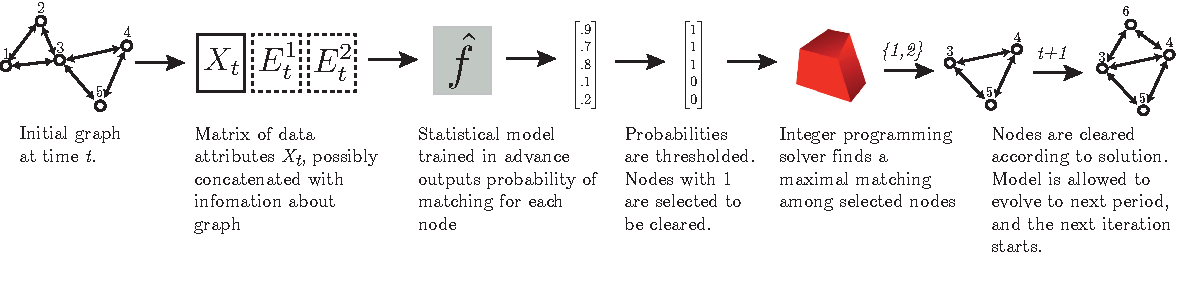
\includegraphics[width=\textwidth]{/Users/vitorhadad/Documents/kidney/matching/phd_thesis/figures/direct_prediction.pdf}.
\caption{\textbf{Direct prediction method} \\ One period of simulation using direct prediction methods to choose cycles. See Algorithm \ref{alg:direct_prediction} for details.}
\label{fig:direct_prediction}
\end{figure}


\begin{algorithm}[htbp]
	\SetAlgoLined
  \DontPrintSemicolon
	
  \KwData{Environment simulator object \textsc{Env}; \\
          Integer programming solver object \textsc{Solver}; \\
          Statistical method \textsc{Classifier} \\
          Threshold $thres$; }

  \SetKwFunction{FChoose}{\textsc{direct\_prediction}}
  \SetKwProg{Fn}{Function}{:}{}
  \Fn{\FChoose{\textsc{Env}, \ \textsc{Solver}, \ \textsc{Classifier}, \ $thres$}}{
    \tcp{Retrieve node (and potentially also graph) data from current environment} \\
    $X, E_1, E_2$ \gets \textsc{Env.get\_data}()  \\
    \tcp{Classifier predicts matching probability for each pair using data} \\
    $prob$ \gets \textsc{Classifier}($X$, \ $E_1$, $E_2$)  \\
    \tcp{Get index of pairs whose probability is higher than threshold} \\
    $index$ $\gets$ \textsc{which}($prob > thres$) \\
    \tcp{Find maximal matching restricted to this subset} \\
    chosen\_cycles $\gets$ \textsc{Solver.solve(Env, subset=$index$)}  \\  
    \tcp{Return chosen cycles to be cleared} \\
    \KwRet chosen\_cycles \;
  }
	\caption{Function \textsc{direct\_prediction}}
	\label{alg:direct_prediction}
\end{algorithm}

\paragraph{Training the classifier} In order to produce data to feed into our ``classifier", we repeatedly created 1000-period simulation runs and solved them offline using \textsc{OPT}. Then, for every period $t$ in simulation $k$, we stored: a matrix $X_t^{k}$ whose rows represent each pairs observable characteristics; an additional matrices $E_{t}^{1k}$ containing additional graph-theoretical information such as several centrality measures (betweenness, in-degree, out-degree, harmonic, closeness), in- and out-degrees, and average neighbor degree; a conforming matrix $E_{t}^{2k}$ containing the entry and death rates used in that simulation; a binary vector $y_t^{k}$ indicating which nodes \textsc{OPT} chose to match in period $t$. Finally, we vertically concatenated each one of these matrices to create the final data set.

We repeated this procedure for each environment, and produced three artificial data sets, each containing approximately 2 million observations. These data sets were then fed to a series of predictive algorithms: penalized logistic regression \citep{wu2009genome}, random forest classifiers \citep{breiman2001random}, and gradient tree boosting classifiers \citep{friedman2001greedy}. 



\subsection{Multi-armed bandit methods}

We have access to the data-generating process (\emph{environments}) and an algorithm that is able to find the best matching for any data in hindsight (\texttt{OPT}). Therefore, in principle we could estimate the best choice of cycle to clear by simulating several periods ahead in the future, running \texttt{OPT}, and measuring the performance of our choice under any desired criterion. 

The approach outlined above turns out to be naive and incomplete, but it essentially contains the insight under which we will be working in this section. It is naive because simulations are computationally expensive, and in practice we cannot repeat them enough times get reliable estimates of the average performance for each cycle choice, especially in large graphs. It is also incomplete because it does not specify exactly what is the best information we should extract from \texttt{OPT} results. In order to solve the first problem, we leverage theory and algorithms from the multi-armed bandit (MAB) literature. For the second, we propose a secondary objective based on what we call \emph{pseudo-rewards}.

Our procedure is illustrated in Figures \ref{fig:mab} and \ref{fig:get_pseudo_reward}. At the beginning of the period $t$, the agent receives a set of cycles $C$ that are available to be cleared. If $C$ is empty, nothing happens and we move to the next period. Otherwise, the agent then picks a cycle $c \in C$ and simulates the future, including new entries and deaths, up to a horizon $h$. Next, \texttt{OPT} is run twice, once normally, and once with the additional constraint that $c$ be removed today. The size of the resulting matching in these two scenarios is compared. Naturally, the constrained version of \texttt{OPT} cannot achieve anything better than its unconstrained counterpart, but it might get to be equal. If it is, the agent receives a \emph{pseudo-reward} of one, otherwise it receives zero. This process is repeated: at each iteration $\ell$, a cycle $c_{\ell}$ is chosen and its pseudo-reward $r_{c, \ell}$ is revealed. When a preset computational budget of $L(|C|)$ iterations is hit, the agent then analyses the whole history of cycle choices and pseudo-rewards $H_{t} = \{ (c_{\ell}, r_{c\ell} ) \}_{\ell=1}^{L}$, and decides whether to match one of the cycles or move on to the next period. If a cycle $c$ is chosen it is immediately cleared, however the environment does not evolve to the next period yet. Instead, the history $H_t$ is discarded the procedure is repeated again with a reduced set of actions $C' \subset C$ that produces a new history $H_t'$ and so on, until either there are no more available choices or the agent decides to allow the environment to move on to time $t+1$. When that at last happens, entries and deaths are revealed, the agent receives a new set of cycles, and the process begin anew. All past information is ignored.


Two important details were left out of the explanation above. First, how does the agent chooses the next cycle to test? Second, how does it decide which cycle to choose (or no cycle at all)? 

Let $c^{*}$ be a cycle that maximizes expected pseudo-rewards during one round of the algorithm:
$$c_{\ell}^{*} \in \arg\max_{c} E[r_{c,\ell}] $$
 Also, let \emph{regret} be defined as the difference between expected reward of the optimal choice $c^*$ and its own selected choice $c_{\ell}$.
 $$\Delta_\ell := E[r_{c^{*},\ell}] - E[r_{c,\ell}]$$
 
 A \emph{multi-armed bandit} (MAB) algorithm is a procedure to minimize the cumulative regret over $L$ rounds. A good MAB algorithm will act so as to balance exploration (trying out different choices to get high-quality estimates of their rewards) and exploitation (using out better choices more often to increase total rewards), and produce regret that grows asymptotically logarithmically with the horizon. Here, we will be experimenting with three common bandits algorithms, named \emph{UCB1}, \emph{EXP3} and \emph{Thompson sampling}.
 
The literature on bandit algorithms is extensive and spans at least seventy years of research, and an in-depth review is outside the score of this paper. We refer the reader to \citep{lattimore2018bandits} for a survey.
 
 
 % Algorithm
 \begin{algorithm}[htbp]
 	\SetAlgoLined
 	\KwData{Cycle $c$; Horizon $h$; \\
           Lists pseudo-reward statistics $Avg$, $Std$; \\
           Environment simulator object \textsc{Env}; \\
           Oracle solver object \textsc{OPT}; }
   \DontPrintSemicolon
   \SetKwFunction{FChoose}{\textsc{get\_pseudo\_reward}}
   \SetKwProg{Fn}{Function}{:}{}
   \Fn{\FChoose{\textsc{Env}, \ $c$, \ $Avg$, \ $Std$, \ $h$ }}{
     \tcp{Simulate up to horizon $h$ and find optimal matching} \\
     \textsc{Env.simulate}($h$)  \\
     $r_1$ \gets \textsc{OPT.solve}(\textsc{Env})  \\
     \tcp{Remove cycle $c$, find constrained optimal matching} \\
     \textsc{Env.remove}($c$)  \\
     $r_2$ \gets \textsc{OPT.solve}(\textsc{Env}) \\
     \tcp{Return 1 if rewards are equal, 0 otherwise} \\
     \KwRet $r_1 == r_2$ \;
   }
 	\caption{Function \textsc{get\_pseudo\_reward}}
 	\label{alg:get_pseudo_reward}
 \end{algorithm}
 
 
 
 \begin{algorithm}[htbp]
 	
   \SetAlgoLined
   \DontPrintSemicolon
 	
   \KwData{Horizon $h$; Number of iterations $L$; Threshold $thres$; \\
     Environment simulator object \textsc{Env};
     Multi-armed bandit algorithm object \textsc{MAB};
   }
 
   \SetKwFunction{FChoose}{\texttt{choose\_cycle}}
   \SetKwProg{Fn}{Function}{:}{}
   
   \Fn{\FChoose{\texttt{Env},\ \texttt{h} }}{
     \tcp{Initialize lists of current pseudo-reward statistics} \\
     $C$ \gets \textsc{Env.get\_available\_cycles()} \\
     $Avg$ \gets \textsc{zeros(length(C))} \\
     $Std$ \gets \textsc{zeros(length(C))} \\
     
     \tcp{Begin iterations} \\
     \For{$i\gets0$ \KwTo $L$}{
       \tcp{Bandit algorithm chooses next cycle to test given statistics} \\
       $c$ \gets \textsc{MAB.pull($C$, Avg, Std)}  \\
       \tcp{Compute pseudo reward for this cycle and update statistics} \\
       $r$ \gets \textsc{get\_pseudo\_reward}(\textsc{Env},\ $c$,\ $Avg$,\ $Std$,\ $h$) \\
       $Avg$ \gets \textsc{update\_running\_average($Avg$, $r$)} \\
       $Std$ \gets \textsc{update\_running\_std($Std$, $r$)} \\ 
     }  
     \tcp{Bandit algorithm chooses best cycle given statistics} \\
     $c\_best$ \gets \textsc{MAB.choose($C$, Avg, Std)} \\
     \tcp{Return best cycle, unless none of the pseudo-reward averages are above a certain threshold} \\
     \eIf{\textsc{All}($Avg \leq thres$)} {
       \KwRet \text{NULL} \\ 
       }{
       \KwRet $c$ \\
       }
     }
   }
 	\caption{Function \texttt{choose\_cycle}}
 	\label{alg:choose_cycle}
 \end{algorithm}


 \begin{figure}[htbp]
  \centering
  %\hspace{-1cm}
  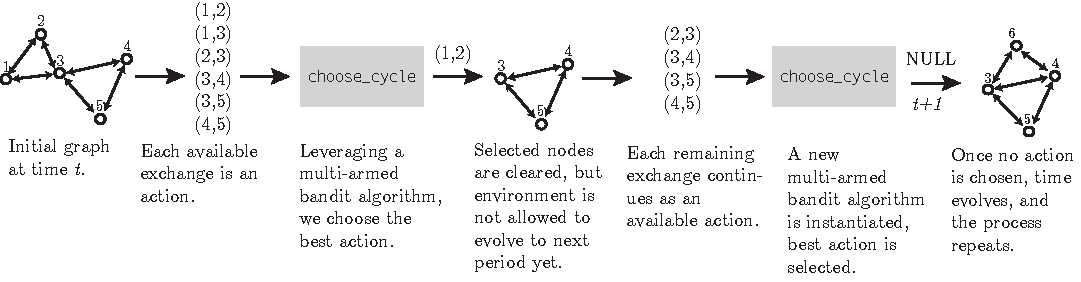
\includegraphics[width=1\textwidth]{/Users/vitorhadad/Documents/kidney/matching/phd_thesis/figures/mab.pdf}
  \caption{\textbf{Multi-armed bandit methods} \\ 
  One period of simulation using multi-armed bandit methods to choose cycles.}
  \label{fig:mab}
  \end{figure}

  \begin{figure}[htbp]
  \centering
  %\hspace*{-0.5cm}
  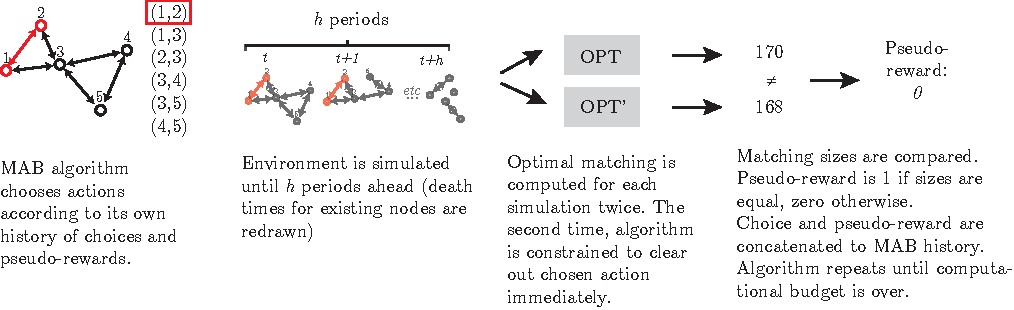
\includegraphics[width=1\textwidth]{/Users/vitorhadad/Documents/kidney/matching/phd_thesis/figures/mab_step.pdf}
  \caption{\textbf{Function} \textsc{get\_pseudo\_reward} \\ Multi-armed bandits evaluate if a cycle should be cleared by checking if there is a high chance that the cycle will be used in the future. Such cycles get a \emph{lower} reward, and are left for later.}
  \label{fig:get_pseudo_reward}
  \end{figure}

\paragraph{What are pseudo-rewards?} As we match and clear out a cycle $c$ today, we forgo the opportunity of using any future cycles involving the nodes in $c$. However, because there may be multiple optimal matchings, sometimes the cycles that become unavailable due to the removal of the nodes in $c$ do not matter, and we can still find a matching of the same cardinality without them. In other words, we pay no price for removing these future cycles.
 
The pseudo-reward associated with cycle $c$ is a random variable whose expectation is the probability that removing a cycle today will \emph{not} negatively impact the optimal matching size between $t$ and $t+h$. The higher this number, the more confident we are that clearing $c$ out today will not give us trouble in the future. A concrete example of this idea in shown in Figure \ref{fig:pseudo_reward_intuition}.

\begin{figure}[htbp]
\centering
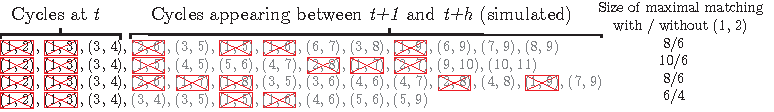
\includegraphics[width=0.95\textwidth]{/Users/vitorhadad/Documents/kidney/matching/phd_thesis/figures/pseudo_reward_intuition.pdf}
\caption{\textbf{Intuition for pseudo-rewards} \\
  In the example above, at time $t$ we have three available cycles to choose from: $(1,2)$, $(1,3)$ and $(3,4)$, and we are contemplating choosing cycle $(1,2)$ at $t$. If we  constrain ourselves to do so, several other future cycles become unavailable (in red). Nevertheless, in three out of our four simulations we were able to clear the same number of cycles in the constrained scenario, so the running pseudo-reward average is $\frac{3}{4}$. 
}
\label{fig:pseudo_reward_intuition}
\end{figure}

Pseudo-rewards are a natural way for us to control which patients should be matched today. Pairs that are easy to match will likely belong to many cycles, so by removing them we will be incurring a large cost in terms of future cycles that will become unavailable. But that means that the pseudo-reward associated with cycles that involve them will be lower, making them less attractive. On the other hand, patients that are harder to match will not participate many future exchange, so the price we pay for matching them today is low, and their average pseudo-reward is high. 



% ---------------------------------------------------------------------------
% Results
% ---------------------------------------------------------------------------

\section{Results}

\subsection{Direct prediction methods} 

Table \ref{tab:traditional_ml_classifier} shows the performance results for direct prediction methods as estimators, i.e., how accurately they are able to predict whether a node should be matched or not. We see that while overall accuracy can be relatively high at 70-80\%, precision (defined as the ratio between true positives and both true and false positives) is low even for simpler environments like $ABO$, indicating that the models are over-predicting matchings. Also, augmenting the data with information about the graph has little discernible effect under any of the performance criteria. This suggests that there might be gains from using other algorithms that make better use of information about the compatibility graph. 

In order to empirically evaluate the performance of our proposed direct prediction method, we proceeded as follow. First, we simulated data using our environments, and applied Algorithm \ref{alg:direct_prediction} at each step, following the outline on Figure \ref{fig:direct_prediction}. Next, using the \emph{same} random seed, we simulated each environment and solved it again using \textsc{Myopic} in lieu of our method. Finally, we computed the average number of matched patients between periods 250 and 1000 (the first 250 periods were used as burn-in) for each algorithm and compared the two. 

This process was repeated several times for: each classifier (logistic regression, gradient tree boosting, random forests), each environment ($ABO$, $RSU$, $OPTN$) and nine entry and death rate combinations. The threshold variable was fixed at $thres = 3$ everywhere.

The result is shown on Figures \ref{fig:traditional_ml_mdp_algo_grb}-\ref{fig:traditional_ml_mdp_algo_rf}, where we show the average performance ratio computed as above for each combination of environment, algorithm and entry/death rate configuration. \footnote{Traditional tables are also available as part of the Supplementary Materials. They will be made available online later.}

Unfortunately, as we predicted in the beginning of the section, the poor predictive performance of the algorithms translates into poor performance as the classifier in our direct prediction method. Random forests, in particular, have the lowest rate of accuracy (Table \ref{tab:traditional_ml_classifier}), and also exhibit the lowest performance in the direct prediction method.


\begin{figure}
\centering
\includegraphics[width=\textwidth]{/Users/vitorhadad/Documents/kidney/matching/phd_thesis/figures/traditional_ml_mdp_algo_grb}
\caption{\textbf{Performance of gradient boosting in direct prediction method} \\
    Ratio of average matched patients against \textsc{Myopic}. Simulations ran over 750 periods (after a 250-period burn-in sequence). Lower row is when data was augmented with information about graph.}
\label{fig:traditional_ml_mdp_algo_grb}
\end{figure}

\begin{figure}
\centering
\includegraphics[width=\textwidth]{/Users/vitorhadad/Documents/kidney/matching/phd_thesis/figures/traditional_ml_mdp_algo_lr}
\caption{\textbf{Performance of logistic regression in direct prediction method} \\
    Similar to gradient boosting shown in Figure \ref{fig:traditional_ml_mdp_algo_grb}, logistic regression is only able to perform better than \textsc{Myopic} when the death rate is large.}
\label{fig:traditional_ml_mdp_algo_lr}
\end{figure}

\begin{figure}
\centering
\includegraphics[width=\textwidth]{/Users/vitorhadad/Documents/kidney/matching/phd_thesis/figures/traditional_ml_mdp_algo_rf}
\caption{\textbf{Performance of random forests in direct prediction method} \\
    Random Forests's poor performance is likely due to its low accuracy (shown on table in online supplement)}
\label{fig:traditional_ml_mdp_algo_rf}
\end{figure}

\subsection{Multi-armed bandit methods}

We evaluated the performance of our \emph{multi-armed bandit} in an analogous manner to the direct prediction method described in the previous section, except that we used Algorithms \ref{alg:choose_cycle} and \ref{alg:get_pseudo_reward} when selecting nodes to be matched at each period.

The average ratio between our method and \textsc{Myopic} is shown on Figure \ref{fig:mab} and elaborated upon on Table \ref{tab:ucb1} in the appendix.\footnote{For reasons of space, in the main paper we present only Table \ref{tab:ucb1}. The remaining tables will be made available in a supplementary online appendix.} The results suggest that, for the entry and death rate combinations we experimented on, the \emph{multi-armed bandit} method uniformly dominates \textsc{Myopic} in terms of average number of matched patients per period.

In sparser environments ($RSU$ and $OPTN$), for particular entry and death rate combinations, our method improve upon \textsc{Myopic} by up to about 4\%. This reflects an earlier observation we did when analyzing Figure \ref{fig:greedy_opt_comparison}: gains from taking dynamic consideration into account are larger in situations of moderate sparsity, because that is where \textsc{Myopic} forces the pool to be too thin, and drives the performance away from optimality.





\begin{figure}
\centering
\hspace*{-1.6cm}
\includegraphics[width=1.1\textwidth]{/Users/vitorhadad/Documents/kidney/matching/phd_thesis/figures/mab_ABO.pdf}
\hspace*{-1.6cm}
\includegraphics[width=1.1\textwidth]{/Users/vitorhadad/Documents/kidney/matching/phd_thesis/figures/mab_RSU.pdf}
\hspace*{-1.6cm}
\includegraphics[width=1.1\textwidth]{/Users/vitorhadad/Documents/kidney/matching/phd_thesis/figures/mab_OPTN.pdf}
\caption{\textbf{Performance multi-armed bandit methods across environments} \\
Average percent improvement by the \emph{multi-armed bandit} method over \textsc{Myopic}. Averages were taken over 750 periods, after a 250-period burn-in sequence. See also Table \ref{tab:ucb1} and additional tables in online supplement. \\
{\scriptsize Note: In $RSU$ row, white entries are missing (they are not zero).}}
\label{fig:mab}
\end{figure}


\section{Conclusion}

In this paper, we examined two novel algorithms for dynamic matching in a discrete-time model of kidney exchange: a \emph{direct prediction method} that tries to predict which pair should be matched at each period; and a \emph{multi-armed bandit method}, that uses simulations to score available exchanges in terms of their desirability. We evaluate these methods them using simulations under a variety of different settings, and compared them in terms of average number of matched pairs per period to a \textsc{Myopic} algorithm that finds and immediately clears the maximal matching at each period.
  
We find that our \emph{multi-armed bandit} method is able to uniformly dominate \textsc{Myopic} in all our simulation settings, including one where we draw pairs from the historical list of patients and donors that have undergone transplants in the United States.

Our methods suggest a variety of extensions. First, the relatively weak performance of our \emph{direct prediction} method could be improved in two ways: by improving our ability to use information about graph structure when predicting if a node should be matched or not; and, by making sure that what we predict for one pair should be dependent on what we predict for the other pairs in the same graph. The former could be done using new statistical methods on non-euclidean spaces \citep{shuman2013emerging}, and the latter using algorithms that output joint distributions of arbitrary length such as recurrent neural networks \citep{lecun2015deep}. We will be turning our attention to these methods next.

Second, while we see that the performance of our \emph{multi-armed bandit} methods was already satisfactory, we note that it uses only simulations and no data to decide which exchange to clear at each period. In that sense, it worked in a diametrically opposite way to the \emph{direct prediction} method that used only data and no simulations. In fact, an intermediate approach, using \emph{contextual bandits} \citep{lattimore2018bandits} could be used, blending information about data and simulations.

Thirdly, we would like to experiment with different objective functions, since, in reality, different exchanges may have different levels of desirability or priority. For example, it is common for pediatric patients and previous organ donors receive higher priority, as do \emph{ABDR0} exchanges involving ``perfectly matched" patients and donors.

Lastly, we remark that there still remains a moderately large gap between what could be optimally achieved if we could perfectly predict the evolution of the pool. It is conceivable that as better predictive methods arise, this gap will become smaller. 



\begin{acks}
	
% The author would like to thank Utku \"{U}nver, Stefan Hoderlein, Arthur Lewbel, Mohammad Akbarpour, Itai Ashlagi, David Parkes, John Dickerson, Enkhmanlai Amarsaikhan and Sainbayar Sukhbaatar for helpful discussions.

The author would like to thank Itai Ashlagi for the idea of a donor cPRA.

This work was supported in part by Health Resources and Services Administration contract 234-2005-37011C. The content is the responsibility of the authors alone and does not necessarily reflect the views or policies of the Department of Health and Human Services, nor does mention of trade names, commercial products, or organizations imply endorsement by the U.S. Government.

	
\end{acks}

% Bibliography
\bibliographystyle{ACM-Reference-Format}
\bibliography{/Users/vitorhadad/Documents/kidney/matching/phd_thesis/references}

\appendix

\section{Tables}



\begin{table}
  \centering
  \singlespacing
  \hspace*{-0.5cm}
  \begin{tabular}{lllrrrr}
\toprule
{} &          Algorithm &   Additional &  Recall (TPR) &  Specificity (TNR) &  Precision &  Accuracy \\
Environment &                    &              &               &                    &            &           \\
\midrule
ABO         &  Gradient boosting &         Both &         0.834 &              0.818 &      0.225 &     0.819 \\
ABO         &  Gradient boosting &    Embedding &         0.841 &              0.826 &      0.234 &     0.826 \\
ABO         &  Gradient boosting &  Graph stats &         0.832 &              0.818 &      0.225 &     0.819 \\
ABO         &  Gradient boosting &         None &         0.838 &              0.827 &      0.237 &     0.828 \\
ABO         &      Logistic reg. &         Both &         0.802 &              0.787 &      0.194 &     0.788 \\
ABO         &      Logistic reg. &    Embedding &         0.735 &              0.797 &      0.188 &     0.793 \\
ABO         &      Logistic reg. &  Graph stats &         0.800 &              0.787 &      0.193 &     0.787 \\
ABO         &      Logistic reg. &         None &         0.734 &              0.798 &      0.188 &     0.794 \\
ABO         &     Random forests &         Both &         0.359 &              0.983 &      0.571 &     0.945 \\
ABO         &     Random forests &    Embedding &         0.423 &              0.973 &      0.496 &     0.940 \\
ABO         &     Random forests &  Graph stats &         0.360 &              0.983 &      0.577 &     0.946 \\
ABO         &     Random forests &         None &         0.745 &              0.854 &      0.244 &     0.847 \\
OPTN        &  Gradient boosting &         Both &         0.592 &              0.830 &      0.436 &     0.787 \\
OPTN        &  Gradient boosting &    Embedding &         0.555 &              0.882 &      0.512 &     0.822 \\
OPTN        &  Gradient boosting &  Graph stats &         0.597 &              0.828 &      0.435 &     0.786 \\
OPTN        &  Gradient boosting &         None &         0.556 &              0.881 &      0.510 &     0.822 \\
OPTN        &      Logistic reg. &         Both &         0.732 &              0.552 &      0.267 &     0.585 \\
OPTN        &      Logistic reg. &    Embedding &         0.760 &              0.552 &      0.274 &     0.590 \\
OPTN        &      Logistic reg. &  Graph stats &         0.730 &              0.553 &      0.266 &     0.585 \\
OPTN        &      Logistic reg. &         None &         0.763 &              0.551 &      0.273 &     0.589 \\
OPTN        &     Random forests &         Both &         0.442 &              0.923 &      0.562 &     0.835 \\
OPTN        &     Random forests &    Embedding &         0.450 &              0.918 &      0.550 &     0.833 \\
OPTN        &     Random forests &  Graph stats &         0.443 &              0.924 &      0.562 &     0.836 \\
OPTN        &     Random forests &         None &         0.448 &              0.913 &      0.534 &     0.828 \\
RSU         &  Gradient boosting &         Both &         0.744 &              0.793 &      0.441 &     0.784 \\
RSU         &  Gradient boosting &    Embedding &         0.732 &              0.810 &      0.457 &     0.796 \\
RSU         &  Gradient boosting &  Graph stats &         0.745 &              0.793 &      0.441 &     0.785 \\
RSU         &  Gradient boosting &         None &         0.732 &              0.812 &      0.460 &     0.798 \\
RSU         &      Logistic reg. &         Both &         0.779 &              0.634 &      0.316 &     0.660 \\
RSU         &      Logistic reg. &    Embedding &         0.778 &              0.629 &      0.314 &     0.656 \\
RSU         &      Logistic reg. &  Graph stats &         0.780 &              0.634 &      0.318 &     0.660 \\
RSU         &      Logistic reg. &         None &         0.777 &              0.629 &      0.313 &     0.656 \\
RSU         &     Random forests &         Both &         0.507 &              0.932 &      0.621 &     0.856 \\
RSU         &     Random forests &    Embedding &         0.500 &              0.930 &      0.609 &     0.853 \\
RSU         &     Random forests &  Graph stats &         0.504 &              0.933 &      0.621 &     0.856 \\
RSU         &     Random forests &         None &         0.732 &              0.797 &      0.441 &     0.786 \\
\bottomrule
\end{tabular}

   \caption{\textbf{Performance of statistical methods as classifiers} \\ 
   We experiment with three variations on the \emph{direct prediction} method by implementing it using different statistical. Here we see their performance as classifiers, that is, how well they are able to predict that the node was chosen to be matched by an offline algorithm. \\
  }
  \label{tab:traditional_ml_classifier}
\end{table}

\begin{table}
  \centering
  \singlespacing
  \hspace*{-0.5cm}
  \begin{tabular}{lllrrrrrrrr}
\toprule
    &     &      & \multicolumn{2}{l}{UCB1} & \multicolumn{2}{l}{Myopic} & Difference & p-value & Ratio (\%) &   N \\
    &     &      &  Mean & Std Error &   Mean & \multicolumn{5}{l}{Std Error} \\
Environ. & Entry & Death &       &           &        &           &            &         &           &     \\
\midrule
ABO & 3.0 & 5.0  & 1.156 &     0.021 &  1.142 &     0.021 &      0.014 &   0.013 &     1.263 &   5 \\
    &     & 8.0  & 1.121 &     0.026 &  1.116 &     0.026 &      0.005 &   0.369 &     0.418 &   3 \\
    &     & 10.0 & 1.095 &     0.020 &  1.079 &     0.020 &      0.016 &   0.003 &     1.484 &   5 \\
    & 5.0 & 5.0  & 2.035 &     0.009 &  2.017 &     0.009 &      0.018 &   0.000 &     0.875 &  63 \\
    &     & 8.0  & 2.021 &     0.031 &  1.996 &     0.031 &      0.025 &   0.004 &     1.237 &   4 \\
    &     & 10.0 & 1.967 &     0.025 &  1.945 &     0.025 &      0.022 &   0.001 &     1.133 &   6 \\
    & 7.0 & 5.0  & 2.908 &     0.050 &  2.894 &     0.050 &      0.014 &   0.048 &     0.497 &   8 \\
    &     & 8.0  & 2.831 &     0.027 &  2.805 &     0.026 &      0.026 &   0.000 &     0.911 &  12 \\
    &     & 10.0 & 2.801 &     0.033 &  2.771 &     0.033 &      0.030 &   0.005 &     1.088 &   5 \\
OPTN & 3.0 & 5.0  & 1.196 &     0.020 &  1.160 &     0.020 &      0.036 &   0.000 &     3.107 &   6 \\
    &     & 8.0  & 1.063 &     0.027 &  1.043 &     0.027 &      0.020 &   0.023 &     1.919 &   3 \\
    &     & 10.0 & 0.998 &     0.020 &  0.971 &     0.019 &      0.027 &   0.002 &     2.763 &   5 \\
    & 5.0 & 5.0  & 2.260 &     0.039 &  2.175 &     0.038 &      0.085 &   0.001 &     3.917 &   4 \\
    &     & 8.0  & 1.981 &     0.025 &  1.914 &     0.025 &      0.066 &   0.000 &     3.469 &   6 \\
    &     & 10.0 & 1.868 &     0.030 &  1.825 &     0.030 &      0.043 &   0.012 &     2.361 &   4 \\
    & 7.0 & 5.0  & 3.398 &     0.020 &  3.264 &     0.020 &      0.134 &   0.000 &     4.106 &  34 \\
    &     & 8.0  & 3.071 &     0.026 &  2.969 &     0.026 &      0.102 &   0.000 &     3.447 &   9 \\
    &     & 10.0 & 2.880 &     0.037 &  2.790 &     0.037 &      0.090 &   0.000 &     3.225 &   5 \\
RSU & 3.0 & 5.0  & 2.477 &     0.026 &  2.398 &     0.026 &      0.078 &   0.000 &     3.268 &   8 \\
    &     & 8.0  & 2.380 &     0.039 &  2.310 &     0.038 &      0.069 &   0.005 &     3.004 &   3 \\
    &     & 10.0 & 2.268 &     0.029 &  2.201 &     0.029 &      0.067 &   0.000 &     3.057 &   5 \\
    & 5.0 & 5.0  & 4.330 &     0.025 &  4.201 &     0.025 &      0.128 &   0.000 &     3.056 &  40 \\
    &     & 8.0  & 4.190 &     0.040 &  4.072 &     0.040 &      0.118 &   0.000 &     2.900 &   8 \\
    &     & 10.0 & 4.084 &     0.011 &  3.973 &     0.011 &      0.112 &   0.000 &     2.815 &  64 \\
    & 7.0 & 5.0  & 5.519 &     0.370 &  5.370 &     0.399 &      0.148 &     nan &     2.759 &   1 \\
    &     & 8.0  & 6.041 &     0.044 &  5.870 &     0.044 &      0.171 &   0.000 &     2.906 &  19 \\
    &     & 10.0 & 5.904 &     0.023 &  5.742 &     0.023 &      0.162 &   0.000 &     2.824 &  53 \\
\bottomrule
\end{tabular}

   \caption{\textbf{Multi-armed bandit algorithm UCB1} \\ 
  \textsc{Environ} is the environment used for simulation. \textsc{Entry} and \textsc{Death} are the Poisson entry rate of entry and the the Geometric rate of departure (times 100), respectively.  \textsc{Mean} and \textsc{Std} refers to the average number of matched patients over 750 periods (after 250 periods of burn-in). \textsc{Difference} and \textsc{Ratio} compare the average improvement between the algorithm and \textsc{Myopic}. \textsc{N} is the number of 1000-period simulations that used that particular configuration. Tables for other bandits are similar, and can be found in the online supplement that will be available online.}
  \label{tab:ucb1}
\end{table}

% 
% 
% \section{Supplementary materials}
% 
% 
% 
% \begin{table}
%   \centering
%   \singlespacing
%   \hspace*{-0.5cm}
%   \begin{tabular}{lllrrrrrrrr}
\toprule
    &     &      & \multicolumn{2}{l}{Thompson} & \multicolumn{2}{l}{Myopic} & Difference & p-value & Ratio (\%) &   N \\
    &     &      &     Mean & Std Error &   Mean & \multicolumn{5}{l}{Std Error} \\
Environ. & Entry & Death &          &           &        &           &            &         &           &     \\
\midrule
ABO & 3.0 & 5.0  &    1.184 &     0.016 &  1.169 &     0.016 &      0.014 &   0.000 &     1.224 &  10 \\
    &     & 8.0  &    1.138 &     0.027 &  1.123 &     0.027 &      0.015 &   0.037 &     1.308 &   3 \\
    &     & 10.0 &    1.114 &     0.017 &  1.102 &     0.017 &      0.012 &   0.019 &     1.116 &   7 \\
    & 5.0 & 5.0  &    2.065 &     0.025 &  2.045 &     0.025 &      0.021 &   0.001 &     1.005 &  12 \\
    &     & 8.0  &    1.999 &     0.017 &  1.982 &     0.017 &      0.017 &   0.000 &     0.835 &  13 \\
    &     & 10.0 &    1.938 &     0.012 &  1.916 &     0.011 &      0.022 &   0.000 &     1.134 &  28 \\
    & 7.0 & 5.0  &    2.861 &     0.058 &  2.837 &     0.058 &      0.024 &   0.026 &     0.836 &   6 \\
    &     & 8.0  &    2.844 &     0.020 &  2.823 &     0.020 &      0.020 &   0.000 &     0.724 &  20 \\
    &     & 10.0 &    2.814 &     0.022 &  2.789 &     0.022 &      0.025 &   0.000 &     0.889 &  12 \\
OPTN & 3.0 & 5.0  &    1.197 &     0.020 &  1.161 &     0.020 &      0.036 &   0.000 &     3.133 &   6 \\
    &     & 8.0  &    1.058 &     0.019 &  1.028 &     0.018 &      0.030 &   0.001 &     2.922 &   6 \\
    &     & 10.0 &    1.000 &     0.025 &  0.980 &     0.025 &      0.021 &   0.031 &     2.112 &   3 \\
    & 5.0 & 5.0  &    2.259 &     0.043 &  2.190 &     0.043 &      0.069 &   0.013 &     3.159 &   3 \\
    &     & 8.0  &    2.023 &     0.022 &  1.962 &     0.021 &      0.061 &   0.000 &     3.098 &   9 \\
    &     & 10.0 &    1.921 &     0.025 &  1.868 &     0.024 &      0.053 &   0.000 &     2.841 &   6 \\
    & 7.0 & 5.0  &    3.393 &     0.019 &  3.263 &     0.019 &      0.131 &   0.000 &     4.009 &  40 \\
    &     & 8.0  &    3.115 &     0.020 &  3.003 &     0.020 &      0.111 &   0.000 &     3.710 &  16 \\
    &     & 10.0 &    2.910 &     0.032 &  2.806 &     0.031 &      0.103 &   0.000 &     3.684 &   6 \\
RSU & 3.0 & 5.0  &    2.447 &     0.025 &  2.364 &     0.025 &      0.084 &   0.000 &     3.542 &   8 \\
    &     & 8.0  &    2.338 &     0.067 &  2.294 &     0.068 &      0.044 &     nan &     1.920 &   1 \\
    &     & 10.0 &    2.250 &     0.038 &  2.198 &     0.038 &      0.052 &   0.009 &     2.369 &   3 \\
    & 5.0 & 5.0  &    4.310 &     0.028 &  4.182 &     0.028 &      0.128 &   0.000 &     3.058 &  32 \\
    &     & 8.0  &    4.145 &     0.035 &  4.013 &     0.035 &      0.133 &   0.000 &     3.305 &  10 \\
    &     & 10.0 &    4.076 &     0.029 &  3.975 &     0.029 &      0.100 &   0.000 &     2.527 &  10 \\
    & 7.0 & 8.0  &    5.971 &     0.044 &  5.801 &     0.044 &      0.170 &   0.000 &     2.926 &  19 \\
    &     & 10.0 &    5.891 &     0.021 &  5.725 &     0.022 &      0.166 &   0.000 &     2.903 &  59 \\
\bottomrule
\end{tabular}

%   \caption{\textbf{Multi-armed bandit algorithm Thompson Sampling} \\ 
%  \textsc{Environ} is the environment used for simulation. \textsc{Entry} and \textsc{Death} are the Poisson entry rate of entry and the the Geometric rate of departure (times 100), respectively.  \textsc{Mean} and \textsc{Std} refers to the average number of matched patients over 750 periods (after 250 periods of burn-in). \textsc{Difference} and \textsc{Ratio} compare the average improvement between the algorithm and \textsc{Myopic}. \textsc{N} is the number of 1000-period simulations that used that particular configuration.}
%   \label{tab:thompson}
% \end{table}
% 
% \begin{table}
%   \centering
%   \singlespacing
%   \hspace*{-0.5cm}
%   \begin{tabular}{lllrrrrrrrr}
\toprule
    &     &      & \multicolumn{2}{l}{EXP3} & \multicolumn{2}{l}{Myopic} & Difference & p-value & Ratio (\%) &   N \\
    &     &      &  Mean & Std Error &   Mean & \multicolumn{5}{l}{Std Error} \\
Environ. & Entry & Death &       &           &        &           &            &         &           &     \\
\midrule
ABO & 3.0 & 5.0  & 1.168 &     0.018 &  1.151 &     0.018 &      0.017 &   0.000 &     1.466 &   7 \\
    &     & 8.0  & 1.108 &     0.019 &  1.096 &     0.019 &      0.012 &   0.014 &     1.127 &   6 \\
    &     & 10.0 & 1.074 &     0.022 &  1.060 &     0.022 &      0.014 &   0.012 &     1.275 &   4 \\
    & 5.0 & 5.0  & 2.035 &     0.010 &  2.016 &     0.010 &      0.019 &   0.000 &     0.952 &  65 \\
    &     & 8.0  & 1.948 &     0.035 &  1.918 &     0.034 &      0.030 &   0.018 &     1.573 &   3 \\
    &     & 10.0 & 1.925 &     0.023 &  1.902 &     0.023 &      0.023 &   0.001 &     1.218 &   7 \\
    & 7.0 & 5.0  & 2.913 &     0.072 &  2.891 &     0.071 &      0.023 &   0.007 &     0.782 &   4 \\
    &     & 8.0  & 2.854 &     0.036 &  2.824 &     0.036 &      0.030 &   0.004 &     1.077 &   7 \\
    &     & 10.0 & 2.815 &     0.034 &  2.788 &     0.034 &      0.027 &   0.007 &     0.966 &   8 \\
OPTN & 3.0 & 5.0  & 1.164 &     0.024 &  1.133 &     0.024 &      0.031 &   0.005 &     2.694 &   4 \\
    &     & 8.0  & 1.037 &     0.023 &  1.012 &     0.022 &      0.026 &   0.005 &     2.524 &   4 \\
    &     & 10.0 & 0.960 &     0.022 &  0.936 &     0.022 &      0.024 &   0.002 &     2.565 &   4 \\
    & 5.0 & 5.0  & 2.301 &     0.044 &  2.236 &     0.043 &      0.065 &   0.027 &     2.890 &   3 \\
    &     & 8.0  & 1.974 &     0.063 &  1.928 &     0.063 &      0.046 &     nan &     2.388 &   1 \\
    &     & 10.0 & 1.850 &     0.030 &  1.806 &     0.030 &      0.044 &   0.014 &     2.438 &   4 \\
    & 7.0 & 5.0  & 3.371 &     0.020 &  3.256 &     0.020 &      0.115 &   0.000 &     3.540 &  35 \\
    &     & 8.0  & 3.056 &     0.027 &  2.961 &     0.027 &      0.095 &   0.000 &     3.206 &   8 \\
    &     & 10.0 & 2.837 &     0.047 &  2.732 &     0.046 &      0.104 &   0.009 &     3.812 &   3 \\
RSU & 3.0 & 5.0  & 2.482 &     0.027 &  2.410 &     0.027 &      0.071 &   0.000 &     2.962 &   7 \\
    &     & 8.0  & 2.361 &     0.008 &  2.304 &     0.008 &      0.057 &   0.000 &     2.462 &  74 \\
    &     & 10.0 & 2.322 &     0.027 &  2.264 &     0.026 &      0.057 &   0.000 &     2.535 &   6 \\
    & 5.0 & 5.0  & 4.277 &     0.027 &  4.155 &     0.027 &      0.122 &   0.000 &     2.941 &  33 \\
    &     & 8.0  & 4.113 &     0.057 &  4.026 &     0.057 &      0.087 &   0.005 &     2.170 &   4 \\
    &     & 10.0 & 4.012 &     0.035 &  3.926 &     0.036 &      0.086 &   0.000 &     2.203 &   8 \\
    & 7.0 & 8.0  & 5.936 &     0.046 &  5.792 &     0.046 &      0.144 &   0.000 &     2.479 &  16 \\
    &     & 10.0 & 5.889 &     0.024 &  5.749 &     0.024 &      0.140 &   0.000 &     2.444 &  51 \\
\bottomrule
\end{tabular}

%   \caption{\textbf{Multi-armed bandit algorithm EXP3} \\ 
%  \textsc{Environ} is the environment used for simulation. \textsc{Entry} and \textsc{Death} are the Poisson entry rate of entry and the the Geometric rate of departure (times 100), respectively.  \textsc{Mean} and \textsc{Std} refers to the average number of matched patients over 750 periods (after 250 periods of burn-in). \textsc{Difference} and \textsc{Ratio} compare the average improvement between the algorithm and \textsc{Myopic}. \textsc{N} is the number of 1000-period simulations that used that particular configuration.}
%   \label{tab:exp3}
% \end{table}
% 
% 
% 
% 
% \begin{table}
%   \centering
%   \singlespacing
%   \hspace*{-0.5cm}
%   \begin{tabular}{lllrrrrrrrr}
\toprule
    &   &    & \multicolumn{2}{l}{Boosting} & \multicolumn{2}{l}{Myopic} & Difference & p-value & Ratio (\%) &   N \\
    &   &    &     Mean & Std Error &   Mean & \multicolumn{5}{l}{Std Error} \\
Environ. & Entry & Death &          &           &        &           &            &         &           &     \\
\midrule
ABO & 3 & 5  &    1.791 &     0.019 &  1.812 &     0.020 &     -0.021 &   0.036 &    -1.173 &  13 \\
    &   & 8  &    2.324 &     0.018 &  2.301 &     0.020 &      0.022 &   0.027 &     0.958 &  15 \\
    &   & 10 &    2.386 &     0.016 &  2.349 &     0.018 &      0.037 &   0.000 &     1.572 &  16 \\
    & 5 & 5  &    2.549 &     0.024 &  2.621 &     0.026 &     -0.072 &   0.000 &    -2.746 &  10 \\
    &   & 8  &    2.870 &     0.018 &  2.880 &     0.020 &     -0.010 &   0.196 &    -0.356 &  16 \\
    &   & 10 &    2.948 &     0.018 &  2.948 &     0.020 &      0.000 &   0.976 &     0.010 &  15 \\
    & 7 & 5  &    3.230 &     0.026 &  3.327 &     0.027 &     -0.097 &   0.000 &    -2.903 &  11 \\
    &   & 8  &    3.531 &     0.026 &  3.575 &     0.028 &     -0.045 &   0.001 &    -1.248 &   9 \\
    &   & 10 &    3.512 &     0.026 &  3.555 &     0.028 &     -0.043 &   0.000 &    -1.209 &   9 \\
OPTN & 3 & 5  &    2.236 &     0.023 &  2.189 &     0.024 &      0.048 &   0.000 &     2.179 &  10 \\
    &   & 8  &    2.314 &     0.016 &  2.259 &     0.017 &      0.055 &   0.000 &     2.431 &  19 \\
    &   & 10 &    2.348 &     0.017 &  2.322 &     0.018 &      0.026 &   0.007 &     1.112 &  18 \\
    & 5 & 5  &    2.347 &     0.026 &  2.515 &     0.027 &     -0.168 &   0.000 &    -6.679 &   9 \\
    &   & 8  &    2.369 &     0.018 &  2.500 &     0.018 &     -0.130 &   0.000 &    -5.210 &  19 \\
    &   & 10 &    2.393 &     0.017 &  2.519 &     0.018 &     -0.126 &   0.000 &    -5.008 &  21 \\
    & 7 & 5  &    3.043 &     0.028 &  3.373 &     0.030 &     -0.330 &   0.000 &    -9.791 &  10 \\
    &   & 8  &    2.900 &     0.030 &  3.192 &     0.032 &     -0.292 &   0.000 &    -9.148 &   8 \\
    &   & 10 &    2.860 &     0.030 &  3.141 &     0.032 &     -0.281 &   0.000 &    -8.957 &   8 \\
RSU & 3 & 5  &    2.380 &     0.025 &  2.417 &     0.025 &     -0.038 &   0.000 &    -1.553 &  10 \\
    &   & 8  &    2.499 &     0.019 &  2.503 &     0.019 &     -0.004 &   0.552 &    -0.155 &  18 \\
    &   & 10 &    2.640 &     0.020 &  2.625 &     0.021 &      0.015 &   0.034 &     0.570 &  16 \\
    & 5 & 5  &    4.193 &     0.031 &  4.247 &     0.031 &     -0.054 &   0.000 &    -1.281 &  12 \\
    &   & 8  &    4.134 &     0.027 &  4.140 &     0.027 &     -0.007 &   0.252 &    -0.163 &  15 \\
    &   & 10 &    4.209 &     0.025 &  4.197 &     0.025 &      0.013 &   0.067 &     0.299 &  17 \\
    & 7 & 5  &    5.987 &     0.039 &  6.037 &     0.040 &     -0.050 &   0.000 &    -0.836 &  10 \\
    &   & 8  &    5.794 &     0.037 &  5.809 &     0.037 &     -0.015 &   0.068 &    -0.260 &  11 \\
    &   & 10 &    5.924 &     0.043 &  5.918 &     0.043 &      0.006 &   0.334 &     0.097 &   8 \\
\bottomrule
\end{tabular}

%    \caption{\textbf{Gradient Boosting (no graph information)} \\ }
%   \label{tab:grb_none}
% \end{table}
% 
% 
% \begin{table}
%   \centering
%   \singlespacing
%   \hspace*{-0.5cm}
%   \begin{tabular}{lllrrrrrrrr}
\toprule
    &   &    & \multicolumn{2}{l}{Boosting} & \multicolumn{2}{l}{Myopic} & Difference & p-value & Ratio (\%) &   N \\
    &   &    &     Mean & Std Error &   Mean & \multicolumn{5}{l}{Std Error} \\
Environ. & Entry & Death &          &           &        &           &            &         &           &     \\
\midrule
ABO & 3 & 5  &    1.827 &     0.023 &  1.874 &     0.024 &     -0.047 &   0.004 &    -2.489 &   9 \\
    &   & 8  &    2.211 &     0.016 &  2.179 &     0.017 &      0.032 &   0.001 &     1.474 &  19 \\
    &   & 10 &    2.292 &     0.016 &  2.254 &     0.017 &      0.039 &   0.000 &     1.713 &  18 \\
    & 5 & 5  &    2.643 &     0.026 &  2.757 &     0.029 &     -0.114 &   0.000 &    -4.131 &   8 \\
    &   & 8  &    2.823 &     0.018 &  2.870 &     0.020 &     -0.046 &   0.000 &    -1.610 &  16 \\
    &   & 10 &    2.915 &     0.020 &  2.914 &     0.021 &      0.000 &   0.937 &     0.011 &  13 \\
    & 7 & 5  &    3.356 &     0.030 &  3.534 &     0.033 &     -0.178 &   0.000 &    -5.039 &   7 \\
    &   & 8  &    3.377 &     0.029 &  3.537 &     0.031 &     -0.160 &   0.000 &    -4.537 &   8 \\
    &   & 10 &    3.432 &     0.028 &  3.516 &     0.030 &     -0.084 &   0.000 &    -2.398 &   8 \\
OPTN & 3 & 5  &    2.131 &     0.023 &  2.127 &     0.024 &      0.004 &   0.695 &     0.192 &  10 \\
    &   & 8  &    2.455 &     0.016 &  2.380 &     0.017 &      0.076 &   0.000 &     3.175 &  17 \\
    &   & 10 &    2.464 &     0.015 &  2.384 &     0.017 &      0.080 &   0.000 &     3.345 &  17 \\
    & 5 & 5  &    2.188 &     0.023 &  2.416 &     0.025 &     -0.228 &   0.000 &    -9.437 &  10 \\
    &   & 8  &    2.812 &     0.017 &  2.825 &     0.019 &     -0.014 &   0.085 &    -0.485 &  19 \\
    &   & 10 &    2.881 &     0.017 &  2.848 &     0.018 &      0.033 &   0.001 &     1.143 &  18 \\
    & 7 & 5  &    2.930 &     0.026 &  3.370 &     0.029 &     -0.440 &   0.000 &   -13.054 &  11 \\
    &   & 8  &    3.139 &     0.025 &  3.358 &     0.028 &     -0.220 &   0.000 &    -6.543 &  11 \\
    &   & 10 &    3.394 &     0.025 &  3.469 &     0.027 &     -0.075 &   0.000 &    -2.162 &  11 \\
RSU & 3 & 5  &    2.380 &     0.025 &  2.451 &     0.025 &     -0.071 &   0.000 &    -2.913 &  10 \\
    &   & 8  &    2.547 &     0.022 &  2.574 &     0.022 &     -0.027 &   0.000 &    -1.044 &  14 \\
    &   & 10 &    2.625 &     0.020 &  2.634 &     0.020 &     -0.009 &   0.148 &    -0.348 &  17 \\
    & 5 & 5  &    4.183 &     0.032 &  4.269 &     0.033 &     -0.086 &   0.000 &    -2.021 &  10 \\
    &   & 8  &    4.179 &     0.026 &  4.211 &     0.027 &     -0.032 &   0.000 &    -0.760 &  15 \\
    &   & 10 &    4.164 &     0.025 &  4.183 &     0.025 &     -0.019 &   0.001 &    -0.449 &  16 \\
    & 7 & 5  &    5.992 &     0.038 &  6.103 &     0.038 &     -0.111 &   0.000 &    -1.813 &  11 \\
    &   & 8  &    5.832 &     0.036 &  5.870 &     0.036 &     -0.039 &   0.000 &    -0.660 &  12 \\
    &   & 10 &    5.914 &     0.037 &  5.939 &     0.037 &     -0.024 &   0.005 &    -0.406 &  11 \\
\bottomrule
\end{tabular}

%    \caption{\textbf{Gradient Boosting (augmented with graph information)} \\ }
%   \label{tab:grb_networkx}
% \end{table}
% 
% 
% \begin{table}
%   \centering
%   \singlespacing
%   \hspace*{-0.5cm}
%   \begin{tabular}{lllrrrrrrrr}
\toprule
    &   &    & \multicolumn{2}{l}{Logistic} & \multicolumn{2}{l}{Myopic} & Difference & p-value & Ratio (\%) &   N \\
    &   &    &     Mean & Std Error &   Mean & \multicolumn{5}{l}{Std Error} \\
Environ. & Entry & Death &          &           &        &           &            &         &           &     \\
\midrule
ABO & 3 & 5  &    1.035 &     0.016 &  1.185 &     0.018 &     -0.150 &   0.000 &   -12.660 &  10 \\
    &   & 8  &    1.479 &     0.015 &  1.530 &     0.015 &     -0.051 &   0.000 &    -3.325 &  19 \\
    &   & 10 &    1.798 &     0.018 &  1.809 &     0.018 &     -0.011 &   0.158 &    -0.594 &  16 \\
    & 5 & 5  &    1.774 &     0.024 &  2.029 &     0.026 &     -0.255 &   0.000 &   -12.556 &   8 \\
    &   & 8  &    1.970 &     0.027 &  2.071 &     0.028 &     -0.101 &   0.000 &    -4.873 &   7 \\
    &   & 10 &    2.275 &     0.021 &  2.328 &     0.021 &     -0.053 &   0.000 &    -2.284 &  13 \\
    & 7 & 5  &    2.536 &     0.033 &  2.908 &     0.036 &     -0.372 &   0.000 &   -12.792 &   6 \\
    &   & 8  &    2.716 &     0.025 &  2.865 &     0.025 &     -0.150 &   0.000 &    -5.219 &  11 \\
    &   & 10 &    2.859 &     0.029 &  2.942 &     0.030 &     -0.083 &   0.000 &    -2.808 &   8 \\
OPTN & 3 & 5  &    1.933 &     0.022 &  1.972 &     0.022 &     -0.039 &   0.004 &    -1.978 &  11 \\
    &   & 8  &    2.270 &     0.017 &  2.232 &     0.019 &      0.038 &   0.000 &     1.712 &  17 \\
    &   & 10 &    2.369 &     0.016 &  2.330 &     0.017 &      0.039 &   0.000 &     1.678 &  17 \\
    & 5 & 5  &    2.717 &     0.027 &  2.795 &     0.029 &     -0.078 &   0.000 &    -2.779 &   9 \\
    &   & 8  &    2.893 &     0.019 &  2.881 &     0.019 &      0.013 &   0.027 &     0.442 &  18 \\
    &   & 10 &    2.922 &     0.019 &  2.879 &     0.020 &      0.043 &   0.000 &     1.490 &  15 \\
    & 7 & 5  &    3.470 &     0.028 &  3.608 &     0.029 &     -0.138 &   0.000 &    -3.832 &  11 \\
    &   & 8  &    3.602 &     0.025 &  3.640 &     0.026 &     -0.038 &   0.000 &    -1.049 &  12 \\
    &   & 10 &    3.611 &     0.026 &  3.606 &     0.027 &      0.005 &   0.470 &     0.148 &  11 \\
RSU & 3 & 5  &    2.037 &     0.025 &  2.434 &     0.027 &     -0.397 &   0.000 &   -16.302 &   9 \\
    &   & 8  &    2.221 &     0.034 &  2.331 &     0.035 &     -0.109 &   0.000 &    -4.688 &   5 \\
    &   & 10 &    2.355 &     0.019 &  2.399 &     0.019 &     -0.044 &   0.000 &    -1.825 &  17 \\
    & 5 & 5  &    3.636 &     0.030 &  4.249 &     0.033 &     -0.613 &   0.000 &   -14.429 &  10 \\
    &   & 8  &    3.886 &     0.028 &  4.080 &     0.028 &     -0.194 &   0.000 &    -4.752 &  14 \\
    &   & 10 &    3.966 &     0.026 &  4.031 &     0.025 &     -0.066 &   0.000 &    -1.634 &  16 \\
    & 7 & 5  &    5.164 &     0.039 &  6.040 &     0.042 &     -0.877 &   0.000 &   -14.512 &   9 \\
    &   & 8  &    5.635 &     0.038 &  5.875 &     0.039 &     -0.240 &   0.000 &    -4.080 &  10 \\
    &   & 10 &    5.606 &     0.038 &  5.706 &     0.038 &     -0.100 &   0.000 &    -1.751 &  10 \\
\bottomrule
\end{tabular}

%    \caption{\textbf{Logistic Regression (no graph information)} \\ }
%   \label{tab:lr_none}
% \end{table}
% 
% 
% \begin{table}
%   \centering
%   \singlespacing
%   \hspace*{-0.5cm}
%   \begin{tabular}{lllrrrrrrrr}
\toprule
    &   &    & \multicolumn{2}{l}{Logistic} & \multicolumn{2}{l}{Myopic} & Difference & p-value & Ratio (\%) &   N \\
    &   &    &     Mean & Std Error &   Mean & \multicolumn{5}{l}{Std Error} \\
Environ. & Entry & Death &          &           &        &           &            &         &           &     \\
\midrule
ABO & 3 & 5  &    1.063 &     0.018 &  1.196 &     0.019 &     -0.133 &   0.000 &   -11.114 &   9 \\
    &   & 8  &    1.350 &     0.017 &  1.405 &     0.017 &     -0.055 &   0.000 &    -3.891 &  14 \\
    &   & 10 &    1.638 &     0.019 &  1.658 &     0.019 &     -0.020 &   0.001 &    -1.186 &  14 \\
    & 5 & 5  &    1.894 &     0.023 &  2.047 &     0.024 &     -0.153 &   0.000 &    -7.452 &   9 \\
    &   & 8  &    2.170 &     0.019 &  2.224 &     0.019 &     -0.054 &   0.000 &    -2.445 &  15 \\
    &   & 10 &    2.430 &     0.019 &  2.439 &     0.019 &     -0.010 &   0.109 &    -0.404 &  17 \\
    & 7 & 5  &    2.745 &     0.034 &  2.963 &     0.035 &     -0.218 &   0.000 &    -7.370 &   6 \\
    &   & 8  &    2.991 &     0.032 &  3.033 &     0.032 &     -0.043 &   0.001 &    -1.403 &   7 \\
    &   & 10 &    3.257 &     0.028 &  3.265 &     0.029 &     -0.008 &   0.290 &    -0.235 &   9 \\
OPTN & 3 & 5  &    1.803 &     0.021 &  1.846 &     0.022 &     -0.043 &   0.025 &    -2.313 &  11 \\
    &   & 8  &    2.302 &     0.018 &  2.263 &     0.019 &      0.039 &   0.000 &     1.733 &  16 \\
    &   & 10 &    2.362 &     0.016 &  2.304 &     0.018 &      0.058 &   0.000 &     2.519 &  16 \\
    & 5 & 5  &    2.519 &     0.027 &  2.642 &     0.028 &     -0.123 &   0.000 &    -4.664 &   9 \\
    &   & 8  &    2.925 &     0.019 &  2.896 &     0.020 &      0.028 &   0.003 &     0.984 &  16 \\
    &   & 10 &    2.956 &     0.018 &  2.908 &     0.019 &      0.048 &   0.000 &     1.643 &  18 \\
    & 7 & 5  &    3.192 &     0.027 &  3.459 &     0.029 &     -0.267 &   0.000 &    -7.716 &  11 \\
    &   & 8  &    3.604 &     0.028 &  3.604 &     0.029 &     -0.000 &   0.940 &    -0.009 &  10 \\
    &   & 10 &    3.654 &     0.024 &  3.617 &     0.025 &      0.037 &   0.000 &     1.014 &  13 \\
RSU & 3 & 5  &    2.062 &     0.023 &  2.424 &     0.024 &     -0.362 &   0.000 &   -14.916 &  11 \\
    &   & 8  &    2.164 &     0.021 &  2.296 &     0.021 &     -0.132 &   0.000 &    -5.760 &  14 \\
    &   & 10 &    2.284 &     0.021 &  2.348 &     0.021 &     -0.065 &   0.000 &    -2.762 &  15 \\
    & 5 & 5  &    3.660 &     0.035 &  4.215 &     0.037 &     -0.555 &   0.000 &   -13.169 &   8 \\
    &   & 8  &    3.876 &     0.028 &  4.061 &     0.027 &     -0.186 &   0.000 &    -4.572 &  15 \\
    &   & 10 &    3.883 &     0.026 &  3.979 &     0.025 &     -0.096 &   0.000 &    -2.424 &  17 \\
    & 7 & 5  &    5.177 &     0.054 &  5.992 &     0.062 &     -0.815 &   0.000 &   -13.596 &   4 \\
    &   & 8  &    5.638 &     0.046 &  5.835 &     0.044 &     -0.197 &   0.000 &    -3.376 &   8 \\
    &   & 10 &    5.688 &     0.043 &  5.787 &     0.041 &     -0.100 &   0.000 &    -1.727 &   9 \\
\bottomrule
\end{tabular}

%    \caption{\textbf{Logistic Regression (augmented with graph information)} \\ }
%   \label{tab:lr_networkx}
% \end{table}
% 
% 
% \begin{table}
%   \centering
%   \singlespacing
%   \hspace*{-0.5cm}
%   \begin{tabular}{lllrrrrrrrr}
\toprule
    &   &    & \multicolumn{2}{l}{Forest} & \multicolumn{2}{l}{Myopic} & Difference & p-value & Ratio (\%) &   N \\
    &   &    &   Mean & Std Error &   Mean & \multicolumn{5}{l}{Std Error} \\
Environ. & Entry & Death &        &           &        &           &            &         &           &     \\
\midrule
ABO & 3 & 5  &  1.173 &     0.019 &  1.240 &     0.020 &     -0.067 &   0.000 &    -5.417 &   8 \\
    &   & 8  &  1.331 &     0.016 &  1.373 &     0.017 &     -0.042 &   0.000 &    -3.082 &  14 \\
    &   & 10 &  1.513 &     0.017 &  1.539 &     0.017 &     -0.026 &   0.002 &    -1.672 &  15 \\
    & 5 & 5  &  1.952 &     0.025 &  2.049 &     0.026 &     -0.097 &   0.000 &    -4.733 &   8 \\
    &   & 8  &  2.223 &     0.019 &  2.281 &     0.020 &     -0.059 &   0.000 &    -2.573 &  15 \\
    &   & 10 &  2.366 &     0.018 &  2.396 &     0.019 &     -0.030 &   0.000 &    -1.240 &  17 \\
    & 7 & 5  &  2.805 &     0.030 &  2.913 &     0.031 &     -0.108 &   0.000 &    -3.715 &   8 \\
    &   & 8  &  2.888 &     0.029 &  2.978 &     0.030 &     -0.089 &   0.000 &    -3.002 &   8 \\
    &   & 10 &  2.990 &     0.025 &  3.049 &     0.026 &     -0.059 &   0.000 &    -1.936 &  11 \\
OPTN & 3 & 5  &  0.962 &     0.018 &  1.256 &     0.020 &     -0.293 &   0.000 &   -23.349 &   8 \\
    &   & 8  &  0.815 &     0.011 &  1.169 &     0.014 &     -0.354 &   0.000 &   -30.298 &  19 \\
    &   & 10 &  0.775 &     0.012 &  1.168 &     0.014 &     -0.394 &   0.000 &   -33.693 &  17 \\
    & 5 & 5  &  1.566 &     0.025 &  2.185 &     0.030 &     -0.619 &   0.000 &   -28.324 &   7 \\
    &   & 8  &  1.269 &     0.014 &  1.969 &     0.018 &     -0.701 &   0.000 &   -35.585 &  17 \\
    &   & 10 &  1.160 &     0.014 &  1.895 &     0.018 &     -0.735 &   0.000 &   -38.766 &  16 \\
    & 7 & 5  &  2.322 &     0.025 &  3.275 &     0.029 &     -0.953 &   0.000 &   -29.110 &  10 \\
    &   & 8  &  1.924 &     0.024 &  2.993 &     0.029 &     -1.069 &   0.000 &   -35.731 &   9 \\
    &   & 10 &  1.736 &     0.024 &  2.807 &     0.030 &     -1.071 &   0.000 &   -38.162 &   8 \\
RSU & 3 & 5  &  2.423 &     0.026 &  2.465 &     0.027 &     -0.043 &   0.000 &    -1.728 &   9 \\
    &   & 8  &  2.670 &     0.022 &  2.664 &     0.022 &      0.006 &   0.368 &     0.213 &  14 \\
    &   & 10 &  2.752 &     0.020 &  2.733 &     0.020 &      0.019 &   0.002 &     0.685 &  17 \\
    & 5 & 5  &  4.175 &     0.037 &  4.214 &     0.037 &     -0.039 &   0.008 &    -0.927 &   8 \\
    &   & 8  &  4.163 &     0.025 &  4.172 &     0.026 &     -0.009 &   0.145 &    -0.213 &  16 \\
    &   & 10 &  4.288 &     0.027 &  4.283 &     0.027 &      0.005 &   0.499 &     0.125 &  15 \\
    & 7 & 5  &  5.996 &     0.052 &  6.042 &     0.052 &     -0.047 &   0.013 &    -0.772 &   6 \\
    &   & 8  &  5.915 &     0.041 &  5.909 &     0.041 &      0.006 &   0.455 &     0.102 &   9 \\
    &   & 10 &  5.827 &     0.036 &  5.820 &     0.036 &      0.007 &   0.481 &     0.121 &  11 \\
\bottomrule
\end{tabular}

%    \caption{\textbf{Random Forests (no graph information)} \\ }
%   \label{tab:rf_none}
% \end{table}
% 
% 
% \begin{table}
%   \centering
%   \singlespacing
%   \hspace*{-0.5cm}
%   \begin{tabular}{lllrrrrrrrr}
\toprule
    &   &    & \multicolumn{2}{l}{Forest} & \multicolumn{2}{l}{Myopic} & Difference & p-value & Ratio (\%) &   N \\
    &   &    &   Mean & Std Error &   Mean & \multicolumn{5}{l}{Std Error} \\
Environ. & Entry & Death &        &           &        &           &            &         &           &     \\
\midrule
ABO & 3 & 5  &  0.953 &     0.017 &  1.181 &     0.018 &     -0.228 &   0.000 &   -19.284 &   9 \\
    &   & 8  &  0.934 &     0.013 &  1.152 &     0.014 &     -0.217 &   0.000 &   -18.874 &  15 \\
    &   & 10 &  0.916 &     0.013 &  1.118 &     0.014 &     -0.202 &   0.000 &   -18.084 &  15 \\
    & 5 & 5  &  1.719 &     0.025 &  2.066 &     0.027 &     -0.347 &   0.000 &   -16.805 &   7 \\
    &   & 8  &  1.645 &     0.017 &  1.938 &     0.018 &     -0.293 &   0.000 &   -15.105 &  16 \\
    &   & 10 &  1.673 &     0.018 &  1.940 &     0.019 &     -0.268 &   0.000 &   -13.796 &  14 \\
    & 7 & 5  &  2.385 &     0.059 &  2.883 &     0.061 &     -0.497 &   0.049 &   -17.253 &   2 \\
    &   & 8  &  2.405 &     0.031 &  2.811 &     0.032 &     -0.406 &   0.000 &   -14.460 &   7 \\
    &   & 10 &  2.424 &     0.027 &  2.819 &     0.028 &     -0.394 &   0.000 &   -13.983 &   9 \\
OPTN & 3 & 5  &  0.517 &     0.012 &  1.180 &     0.018 &     -0.663 &   0.000 &   -56.214 &  10 \\
    &   & 8  &  0.552 &     0.010 &  1.087 &     0.014 &     -0.535 &   0.000 &   -49.181 &  17 \\
    &   & 10 &  0.619 &     0.010 &  1.111 &     0.013 &     -0.491 &   0.000 &   -44.245 &  18 \\
    & 5 & 5  &  0.946 &     0.018 &  2.161 &     0.027 &     -1.215 &   0.000 &   -56.221 &   8 \\
    &   & 8  &  0.909 &     0.012 &  1.962 &     0.018 &     -1.053 &   0.000 &   -53.661 &  17 \\
    &   & 10 &  0.963 &     0.012 &  1.873 &     0.017 &     -0.910 &   0.000 &   -48.590 &  17 \\
    & 7 & 5  &  2.173 &     0.028 &  3.313 &     0.032 &     -1.141 &   0.000 &   -34.424 &   9 \\
    &   & 8  &  1.314 &     0.017 &  2.993 &     0.026 &     -1.679 &   0.000 &   -56.088 &  12 \\
    &   & 10 &  1.344 &     0.017 &  2.822 &     0.025 &     -1.479 &   0.000 &   -52.392 &  12 \\
RSU & 3 & 5  &  2.102 &     0.025 &  2.372 &     0.027 &     -0.270 &   0.000 &   -11.369 &   9 \\
    &   & 8  &  2.074 &     0.019 &  2.304 &     0.020 &     -0.229 &   0.000 &    -9.957 &  15 \\
    &   & 10 &  2.087 &     0.018 &  2.301 &     0.019 &     -0.215 &   0.000 &    -9.322 &  16 \\
    & 5 & 5  &  3.859 &     0.032 &  4.243 &     0.033 &     -0.385 &   0.000 &    -9.064 &  10 \\
    &   & 8  &  3.744 &     0.025 &  4.070 &     0.026 &     -0.325 &   0.000 &    -7.998 &  15 \\
    &   & 10 &  3.666 &     0.020 &  3.976 &     0.021 &     -0.311 &   0.000 &    -7.815 &  23 \\
    & 7 & 5  &  5.564 &     0.052 &  6.027 &     0.051 &     -0.464 &   0.000 &    -7.693 &   6 \\
    &   & 8  &  5.455 &     0.041 &  5.821 &     0.043 &     -0.365 &   0.000 &    -6.277 &   8 \\
    &   & 10 &  5.427 &     0.042 &  5.762 &     0.043 &     -0.335 &   0.000 &    -5.816 &   8 \\
\bottomrule
\end{tabular}

%    \caption{\textbf{Random Forests (augmented with graph information)} \\ }
%   \label{tab:rf_networkx}
% \end{table}
% 







\end{document}
